\chapter{Quantum walk}

Classical random graph walks can be seen as using a classical coin flip to decide in the current vertex which neighbouring vertex to step next. To create a quantum version of these walks, we define the quantum coin to randomize the walk, then use entanglement between the coin and the register of the current vertex, to influence stepping.

A great introduction to quantum walks is in Portugal's Quantum Walks and Search Algorithms book \cite{Portugal}.

\section{Definition of the quantum coin}

The quantum coin has a current state, which according to Postulate 1 and 4 is an n-qubit register and a transition operator, which according to Postulate 2 is a unitary matrix.

The current state decides where to step next. If there are $d$ neighbours to choose from, the coin's current state register must be $d$ dimensional.

The transition operator decides how the coin is flipped. If the coin is $d$ dimensional, the transition operator is a $d\times{}d$ dimensional matrix. Based on what the transition operator is, multiple types of coins can be defined. The following ones are typically used in quantum walks.

\definition{\textbf{Hadamard coin}}

The Hadamard coin uses the Hadamard-matrix as a transition operator, which is the following:

\begin{align}
  H = \frac{1}{\sqrt{2}}\begin{pmatrix}
      1 & 1  \\
      1 & -1
    \end{pmatrix}
\end{align}

If the starting coin state is $\ket{0}$, then flipping the coin once results in the following state:

\begin{align}
 H\ket{0} = \frac{1}{\sqrt{2}}\begin{pmatrix}
      1 & 1  \\
      1 & -1
    \end{pmatrix} \begin{pmatrix} 1 \\ 0 \end{pmatrix}
    = \frac{1}{\sqrt{2}} \begin{pmatrix} 1 \\ 1 \end{pmatrix} = \frac{1}{\sqrt{2}} \ket{0} + \frac{1}{\sqrt{2}} \ket{1}
\end{align}

If we measured the above coin, the probability of measuring $\ket{0}$ is $\left\lvert\frac{1}{\sqrt{2}}\right\rvert^2 + \left\lvert\frac{1}{\sqrt{2}}\right\rvert^2 = \frac{1}{2}$.

Similarly the starting coin state is $\ket{1}$, then flipping the coin once results in the following state:

\begin{align}
   H\ket{1} = \frac{1}{\sqrt{2}}\begin{pmatrix}
      1 & 1  \\
      1 & -1
    \end{pmatrix} \begin{pmatrix} 0 \\ 1 \end{pmatrix}
    = \frac{1}{\sqrt{2}} \begin{pmatrix} 1 \\ -1 \end{pmatrix} = \frac{1}{\sqrt{2}} \ket{0} - \frac{1}{\sqrt{2}} \ket{1}
\end{align}

the probability of measuring $\ket{1}$ is similarly $\left\lvert\frac{1}{\sqrt{2}}\right\rvert^2 + \left\lvert-\frac{1}{\sqrt{2}}\right\rvert^2 = \frac{1}{2}$.

An interesting property about this coin is related to the fact, that the Hadamard-matrix is Hermitian (self-adjoint), i.e. $H^{\dagger} = H$, while also unitary, i.e. $H^{\dagger} = H^{-1}$, which results in $H^{-1} = H$, thus $HH = I$. This means, that if we flip the coin twice, without measuring it, it will return to its original state, for example:

\begin{align}
 H^2 \ket{0} = H\frac{1}{\sqrt{2}}(\ket{0} + \ket{1}) = \frac{1}{2}(\ket{0} + \ket{1} + \ket{0} - \ket{1}) = \ket{0}
\end{align}

After the second flip, the probability of measuring $\ket{0}$ is 1, due to the destrutive interference between the $\ket{1}$ vectors. This illustrates the vast difference between classical and quantum walks.

\definition{\textbf{$2^n$ dimensional Hadamard-coin}}: A $2^n$ dimensional Hadamard-coin can be created by taking the tensor product of the $2$ dimensional Hadamard-coin $n$ times: $H^{\otimes{}n}$



\definition{\textbf{Grover coin}}

The Grover coin's origin is the Grover search algorithm, where it is used as the diffusion operator, defined as follows:

The diagonal state of the coin space:

\begin{align}
    \ket{D} = H^{\otimes{}n}\ket{0} = \frac{1}{\sqrt{2^n}} \sum\limits_{i=0}^{2^n-1} \ket{i}
\end{align}

Grover coin:

\begin{align}
    G = 2\ket{D}\bra{D} - I
\end{align}

If $N = 2^n$, then

\begin{align}
  G = \begin{pmatrix}
      \frac{2}{N} - 1 & \frac{2}{N} & \dots  & \frac{2}{N} \\
      \frac{2}{N} & \frac{2}{N} - 1 & \dots  & \frac{2}{N} \\
      \vdots & \vdots & \ddots & \vdots \\
      \frac{2}{N} & \frac{2}{N} & \ddots & \frac{2}{N} - 1
    \end{pmatrix}
\end{align}

\paragraph{Fourier coin}

While both the Hadamard and the Fourier coin need to be sized as a power of $2$, the Fourier coin does not have this limitation. A size $N$ Fourier-coin, $F_N$ is defined by the matrix of the Fourier-transform:

\unsure{A Quanutm diszkrét Fourier transzformáció mátrixa talán ez?}

\begin{align}
[F_N]_{k,l} = \frac{1}{\sqrt{N}} \omega^{kl}
\end{align}

where 
\begin{align}
    \omega = e^{\frac{2\pi{}i}{N}}
\end{align}

\begin{align}
  F_N = \frac{1}{\sqrt{N}}\begin{pmatrix}
      1 &  1 & \dots  & 1 \\
      1 &  e^{\frac{2\pi{}i}{N}} & \dots  & e^{\frac{2\pi{}i(N-1)}{N}} \\
      \vdots & \vdots & \ddots & \vdots \\
      1 &  e^{\frac{2\pi{}i(N-1)}{N}} & \ddots & e^{\frac{2\pi{}i(N-1)^2}{N}}
    \end{pmatrix}
\end{align}

\section{Quantum walks on the line}

\change{Ez az önlabomból van, picit rövidítve be lehetne tenni ide.}

The simplest form of a quantum walk to discuss is the quantum walk on the line. A great introduction into this is in \cite{KempeIntroduction}.

A line is an infinite 2-regular graph

A kvantumbolyongásokat 2-reguláris gráfok esetén tehát a Hadamard-mátrix
segítségével definiáljuk. A következőkben az egyenesen, mint 2-reguláris gráfon
vett bolyongást fogjuk részletesen megvizsgálni. Ez a fejezet Susan Stepney
Quantum walking című írása \cite{Stepney} alapján készült.

Tegyük fel, hogy a bolyongás az egyenesen az origóból indul és a $k.$ lépés
után megáll. Ekkor a pozíció tárolására elegendő egy $(2k+1)$ méretű
állapotvektor, hiszen legfeljebb $k$ messzire juthatunk mindkét irányban a
kezdőponttól. Jelöljük ezt $\ket{P}$-vel és legyen $\ket{P}=(p_{-k}, ..., p_0,
  ..., p_{k})$, ahol $p_i\in\mathds{C}$ $\forall i$-re és $\sum\limits_{i=-k}^{k}
  |p_i|^2 = 1$. Azt mondjuk, hogy annak a valószínűsége, hogy a bolyongó éppen az
$i.$ koordinátán van $|p_i|^2$. Ezáltal egy teljes valószínűségi eloszlást
kaptunk a bolyongó pozíciója szerint.

Mivel kezdetben a bolyongó az origóban van, ezért a hozzá tartozó állapotvektor
$\ket{P_0} = (0, ..., 0, 1, 0, ..., 0)$, vagyis $p_0=1$, a többi $0$. A kvantumérme
kiindulási állapota pedig legyen $\ket{C_0} = \begin{pmatrix} \frac{1}{\sqrt{2}} \\
    \frac{i}{\sqrt{2}}\end{pmatrix}$. Ekkor a teljes rendszer állapotát e kettő
tenzorszorzata fogja megadni:

\begin{center}
  $\ket{\Psi_0} = \ket{P_0} \otimes \ket{C_0}
    = \frac{1}{\sqrt{2}} \begin{pmatrix}
      p_{-k}         \\
      i\cdot{}p_{-k} \\
      \vdots         \\
      p_{0}          \\
      i\cdot{}p_{0}  \\
      \vdots         \\
      p_{k}          \\
      i\cdot{}p_{k}
    \end{pmatrix}
  $
\end{center}

A lépés ezek után két fázisból áll. Az első fázisban az érmével dobunk. Ahhoz, hogy
a $\ket{\Psi}$ vektorban az érme állapotát frissítsük, azt az $I_{2k+1} \otimes H$
mátrixszal kell beszorozni. Ez egy olyan $(4k+2) \times (4k+2)$ -es mátrix, mely
$2 \times 2$-es almátrixokból áll és az átlójában Hadamard-mátrixok vannak:

\begin{center}
  \[ \hat{C} =
    \left(
    \begin{array}{cc|cc|cc|cc|cc|cc|cc}
        \frac{1}{\sqrt{2}} & \frac{1}{\sqrt{2}}  & 0      & 0      & \dots              & \dots               & \dots              & \dots               & \dots              & \dots               & \dots  & \dots  & 0                  & 0                   \\
        \frac{1}{\sqrt{2}} & -\frac{1}{\sqrt{2}} & 0      & 0      & \dots              & \dots               & \dots              & \dots               & \dots              & \dots               & \dots  & \dots  & 0                  & 0                   \\ \hline
        0                  & 0                   & \ddots &        & \ddots             &                     & \ddots             &                     & \ddots             &                     & \ddots &        & \vdots             & \vdots              \\
        0                  & 0                   &        & \ddots &                    & \ddots              &                    & \ddots              &                    & \ddots              &        & \ddots & \vdots             & \vdots              \\ \hline
        \vdots             & \vdots              & \ddots &        & \frac{1}{\sqrt{2}} & \frac{1}{\sqrt{2}}  & 0                  & 0                   & \ddots             &                     & \ddots &        & \vdots             & \vdots              \\
        \vdots             & \vdots              &        & \ddots & \frac{1}{\sqrt{2}} & -\frac{1}{\sqrt{2}} & 0                  & 0                   &                    & \ddots              &        & \ddots & \vdots             & \vdots              \\ \hline
        \vdots             & \vdots              & \ddots &        & 0                  & 0                   & \frac{1}{\sqrt{2}} & \frac{1}{\sqrt{2}}  & 0                  & 0                   & \ddots &        & \vdots             & \vdots              \\
        \vdots             & \vdots              &        & \ddots & 0                  & 0                   & \frac{1}{\sqrt{2}} & -\frac{1}{\sqrt{2}} & 0                  & 0                   &        & \ddots & \vdots             & \vdots              \\ \hline
        \vdots             & \vdots              & \ddots &        & \ddots             &                     & 0                  & 0                   & \frac{1}{\sqrt{2}} & \frac{1}{\sqrt{2}}  & \ddots &        & \vdots             & \vdots              \\
        \vdots             & \vdots              &        & \ddots &                    & \ddots              & 0                  & 0                   & \frac{1}{\sqrt{2}} & -\frac{1}{\sqrt{2}} &        & \ddots & \vdots             & \vdots              \\ \hline
        \vdots             & \vdots              & \ddots &        & \ddots             &                     & \ddots             &                     & \ddots             &                     & \ddots &        & 0                  & 0                   \\
        \vdots             & \vdots              &        & \ddots &                    & \ddots              &                    & \ddots              &                    & \ddots              &        & \ddots & 0                  & 0                   \\ \hline
        0                  & 0                   & \dots  & \dots  & \dots              & \dots               & \dots              & \dots               & \dots              & \dots               & 0      & 0      & \frac{1}{\sqrt{2}} & \frac{1}{\sqrt{2}}  \\
        0                  & 0                   & \dots  & \dots  & \dots              & \dots               & \dots              & \dots               & \dots              & \dots               & 0      & 0      & \frac{1}{\sqrt{2}} & -\frac{1}{\sqrt{2}} \\
      \end{array}
    \right)
  \]
\end{center}

A második fázisban a gráfon lépünk a következő csúcsba. Ahhoz, hogy balra lépjünk
a pozíció állapotvektorát egy olyan $S_{-}$ mátrixszal kell megszorozni, ami
az átló feletti 1-eseket tartalmaz:

\begin{center}
  \[ S_{-} =
    \left(
    \begin{array}{ccccc}
        0      & 1      & 0      & \cdots & 0      \\
               & \ddots & \ddots & \ddots & \vdots \\
        \vdots &        & \ddots & \ddots & 0      \\
               &        &        & \ddots & 1      \\
        0      &        & \cdots &        & 0
      \end{array}
    \right)
  \]
\end{center}

Ahhoz pedig, hogy jobbra lépjünk, egy olyan $S_{+}$ mátrixszal kell szorozni,
ami az átló alatti 1-eseket tartalmaz:

\begin{center}
  \[ S_{+} =
    \left(
    \begin{array}{ccccc}

        0      &        & \cdots &        & 0      \\
        1      & \ddots &        &        &        \\
        0      & \ddots & \ddots &        & \vdots \\
        \vdots & \ddots & \ddots & \ddots &        \\
        0      & \cdots & 0      & 1      & 0
      \end{array}
    \right)
  \]
\end{center}

Az érme $\ket{0}$ értékére lépünk balra, az $\ket{1}$ értékére pedig jobbra.
Tehát

\begin{center}
  \[ \hat{S} = S_{-}\otimes\ket{0}\bra{0} + S_{+}\otimes\ket{1}\bra{1}
  \]
\end{center}

Ami kifejtve,

\begin{center}
  \[ \hat{S} =
    \left(
    \begin{array}{cc|cc|cc|cc|cc|cc|cc}
        0                    & 0                    & \cellcolor{green!10} 1 & \cellcolor{green!10} 0 & 0                    & 0                    & \dots                  & \dots                  & \dots                  & \dots                  & \dots                & \dots                & 0                      & 0                      \\
        0                    & 0                    & \cellcolor{green!10} 0 & \cellcolor{green!10} 0 & 0                    & 0                    & \dots                  & \dots                  & \dots                  & \dots                  & \dots                & \dots                & 0                      & 0                      \\ \hline
        \cellcolor{red!10} 0 & \cellcolor{red!10} 0 & \ddots                 &                        & \ddots               &                      & \ddots                 &                        & \ddots                 &                        & \ddots               &                      & \vdots                 & \vdots                 \\
        \cellcolor{red!10} 0 & \cellcolor{red!10} 1 &                        & \ddots                 &                      & \ddots               &                        & \ddots                 &                        & \ddots                 &                      & \ddots               & \vdots                 & \vdots                 \\ \hline
        0                    & 0                    & \ddots                 &                        & 0                    & 0                    & \cellcolor{green!10} 1 & \cellcolor{green!10} 0 & \ddots                 &                        & \ddots               &                      & \vdots                 & \vdots                 \\
        0                    & 0                    &                        & \ddots                 & 0                    & 0                    & \cellcolor{green!10} 0 & \cellcolor{green!10} 0 &                        & \ddots                 &                      & \ddots               & \vdots                 & \vdots                 \\ \hline
        \vdots               & \vdots               & \ddots                 &                        & \cellcolor{red!10} 0 & \cellcolor{red!10} 0 & 0                      & 0                      & \cellcolor{green!10} 1 & \cellcolor{green!10} 0 & \ddots               &                      & \vdots                 & \vdots                 \\
        \vdots               & \vdots               &                        & \ddots                 & \cellcolor{red!10} 0 & \cellcolor{red!10} 1 & 0                      & 0                      & \cellcolor{green!10} 0 & \cellcolor{green!10} 0 &                      & \ddots               & \vdots                 & \vdots                 \\ \hline
        \vdots               & \vdots               & \ddots                 &                        & \ddots               &                      & \cellcolor{red!10} 0   & \cellcolor{red!10} 0   & 0                      & 0                      & \ddots               &                      & 0                      & 0                      \\
        \vdots               & \vdots               &                        & \ddots                 &                      & \ddots               & \cellcolor{red!10} 0   & \cellcolor{red!10} 1   & 0                      & 0                      &                      & \ddots               & 0                      & 0                      \\ \hline
        \vdots               & \vdots               & \ddots                 &                        & \ddots               &                      & \ddots                 &                        & \ddots                 &                        & \ddots               &                      & \cellcolor{green!10} 1 & \cellcolor{green!10} 0 \\
        \vdots               & \vdots               &                        & \ddots                 &                      & \ddots               &                        & \ddots                 &                        & \ddots                 &                      & \ddots               & \cellcolor{green!10} 0 & \cellcolor{green!10} 0 \\ \hline
        0                    & 0                    & \dots                  & \dots                  & \dots                & \dots                & \dots                  & \dots                  & 0                      & 0                      & \cellcolor{red!10} 0 & \cellcolor{red!10} 0 & 0                      & 0                      \\
        0                    & 0                    & \dots                  & \dots                  & \dots                & \dots                & \dots                  & \dots                  & 0                      & 0                      & \cellcolor{red!10} 0 & \cellcolor{red!10} 1 & 0                      & 0                      \\
      \end{array}
    \right)
  \]
\end{center}

A két fázist összevonva egy lépéshez a következő mátrix tartozik:

\begin{center}
  \[ \hat{U} = \hat{S} \cdot \hat{C} =
    (S_{-}\otimes\ket{0}\bra{0} + S_{+}\otimes\ket{1}\bra{1})\cdot\hat{C}
  \]
\end{center}

Ami kifejtve,

\begin{center}
  \[ \hat{U} =
    \left(
    \begin{array}{cc|cc|cc|cc|cc|cc|cc}
        0                    & 0                                      & \cellcolor{green!10} \frac{1}{\sqrt{2}} & \cellcolor{green!10} 0 & 0                    & 0                                      & \dots                                   & \dots                                  & \dots                                   & \dots                  & \dots                & \dots                                  & 0                                       & 0                      \\
        0                    & 0                                      & \cellcolor{green!10} \frac{1}{\sqrt{2}} & \cellcolor{green!10} 0 & 0                    & 0                                      & \dots                                   & \dots                                  & \dots                                   & \dots                  & \dots                & \dots                                  & 0                                       & 0                      \\ \hline
        \cellcolor{red!10} 0 & \cellcolor{red!10} \frac{1}{\sqrt{2}}  & \ddots                                  &                        & \ddots               &                                        & \ddots                                  &                                        & \ddots                                  &                        & \ddots               &                                        & \vdots                                  & \vdots                 \\
        \cellcolor{red!10} 0 & \cellcolor{red!10} -\frac{1}{\sqrt{2}} &                                         & \ddots                 &                      & \ddots                                 &                                         & \ddots                                 &                                         & \ddots                 &                      & \ddots                                 & \vdots                                  & \vdots                 \\ \hline
        0                    & 0                                      & \ddots                                  &                        & 0                    & 0                                      & \cellcolor{green!10} \frac{1}{\sqrt{2}} & \cellcolor{green!10} 0                 & \ddots                                  &                        & \ddots               &                                        & \vdots                                  & \vdots                 \\
        0                    & 0                                      &                                         & \ddots                 & 0                    & 0                                      & \cellcolor{green!10} \frac{1}{\sqrt{2}} & \cellcolor{green!10} 0                 &                                         & \ddots                 &                      & \ddots                                 & \vdots                                  & \vdots                 \\ \hline
        \vdots               & \vdots                                 & \ddots                                  &                        & \cellcolor{red!10} 0 & \cellcolor{red!10} \frac{1}{\sqrt{2}}  & 0                                       & 0                                      & \cellcolor{green!10} \frac{1}{\sqrt{2}} & \cellcolor{green!10} 0 & \ddots               &                                        & \vdots                                  & \vdots                 \\
        \vdots               & \vdots                                 &                                         & \ddots                 & \cellcolor{red!10} 0 & \cellcolor{red!10} -\frac{1}{\sqrt{2}} & 0                                       & 0                                      & \cellcolor{green!10} \frac{1}{\sqrt{2}} & \cellcolor{green!10} 0 &                      & \ddots                                 & \vdots                                  & \vdots                 \\ \hline
        \vdots               & \vdots                                 & \ddots                                  &                        & \ddots               &                                        & \cellcolor{red!10} 0                    & \cellcolor{red!10} \frac{1}{\sqrt{2}}  & 0                                       & 0                      & \ddots               &                                        & 0                                       & 0                      \\
        \vdots               & \vdots                                 &                                         & \ddots                 &                      & \ddots                                 & \cellcolor{red!10} 0                    & \cellcolor{red!10} -\frac{1}{\sqrt{2}} & 0                                       & 0                      &                      & \ddots                                 & 0                                       & 0                      \\ \hline
        \vdots               & \vdots                                 & \ddots                                  &                        & \ddots               &                                        & \ddots                                  &                                        & \ddots                                  &                        & \ddots               &                                        & \cellcolor{green!10} \frac{1}{\sqrt{2}} & \cellcolor{green!10} 0 \\
        \vdots               & \vdots                                 &                                         & \ddots                 &                      & \ddots                                 &                                         & \ddots                                 &                                         & \ddots                 &                      & \ddots                                 & \cellcolor{green!10} \frac{1}{\sqrt{2}} & \cellcolor{green!10} 0 \\ \hline
        0                    & 0                                      & \dots                                   & \dots                  & \dots                & \dots                                  & \dots                                   & \dots                                  & 0                                       & 0                      & \cellcolor{red!10} 0 & \cellcolor{red!10} \frac{1}{\sqrt{2}}  & 0                                       & 0                      \\
        0                    & 0                                      & \dots                                   & \dots                  & \dots                & \dots                                  & \dots                                   & \dots                                  & 0                                       & 0                      & \cellcolor{red!10} 0 & \cellcolor{red!10} -\frac{1}{\sqrt{2}} & 0                                       & 0                      \\
      \end{array}
    \right)
  \]
\end{center}

Az $i.$ lépés után tehát az aktuális $\Psi$ állapotvektor: $\ket{\Psi_i} =
  {\hat{U}}^i\cdot{}\ket{\Psi_0}$.

\paragraph{Mérés}

Annak a mérése, hogy a $i.$ koordinátán mekkora valószínűséggel van a bolyongó
a $j.$ lépésben.

Legyen $e_i$ egy $(2k+1)$ méretű csupa-0 vektor, kivéve az $i.$ koordinátát,
ahol 1 az értéke. Ekkor az állapotvektorból az i. koordinátához tartozó blokkot
az $\ket{e_i}\bra{e_i} \otimes \begin{pmatrix} 1 & 0 \\ 0 & 1 \end{pmatrix}$
mátrixszal történő beszorzással lehet kivágni:

\begin{center} \[ \ket{\phi_{i,j}} =
    (\ket{e_i}\bra{e_i} \otimes
    \begin{pmatrix} 1 & 0 \\ 0 & 1 \end{pmatrix})
    \cdot{} \ket{\Psi_j} \]
\end{center}

A blokkhoz tartozó valószínűség értéke az önmagával vett
(komplex) skalárszorzatának az eredménye lesz, azaz $\braket{\phi_{i,j}}$, ami valós.

Az ebben a fejezetben bemutatott algoritmust implementáltam a félév során. A 6.
fejezetben részletesen ismertetem az ezzel kapcsolatos szimulációs
eredményeket.

\section{Kvantumséta a rácson}

A következőkben a rácson, mint 4-reguláris gráfon vett bolyongást fogjuk
részletesen megvizsgálni.

Legyen a rács $N = n \times n$ -es.

Pozíció vektor: $\ket{P} =  (p_{0}, \dots, p_{N})$, ahol
$p_{i}\in\mathds{C}$ ahol $0 \leq{} i < N$, $\forall{}i$-re és $\sum\limits_{i=0}^{N} |p_i|^2 = 1$.

\begin{align}
  \ket{P_{0}} =  (0, \dots, 0, 1, 0, \dots, 0)
\end{align}

\begin{align}
  C = (\frac{1}{\sqrt{2}}, \frac{i}{\sqrt{2}}) \otimes (\frac{1}{\sqrt{2}}, \frac{i}{\sqrt{2}})
\end{align}

\begin{align}
  S_{\text{left}} =
  \begin{pmatrix}
    0      & 0      & 0      & \dots  & 0 \\
    1      & 0      & 0      & \dots  & 0 \\
    0      & 1      & 0      & \ddots & 0 \\
    \vdots & \ddots & \ddots & 0
  \end{pmatrix}
\end{align}

% https://hu.wikipedia.org/wiki/Kronecker_delta_f%C3%BCggv%C3%A9ny
\begin{definition}[Kronecker delta]
  Olyan kétváltozós függvény ami akkor $1$, ha a két változója egyenlő, egyébként $0$.
  \begin{align}
    \delta_{ij} =
    \begin{cases}
      0 & \text{ha $i\neq{}j$} \\
      1 & \text{ha $i=j$}
    \end{cases}
  \end{align}
\end{definition}

% https://en.wikipedia.org/wiki/Shift_matrix
\begin{definition}[Upper cyclic shift matrix]
  Az $U_{k}$ mátrix egy olyan ($k\times{}k$)-s mátrix, aminek a felső mellékátlóján és a bal alsó sarokban
  $1$-esek vannak, máshol $0$-k.
  Az index számozása moduló k történik.
  Ennek az $i$. sor, $j$. oszlopában:
  \begin{align}
    U_{k}[i,j] = \delta_{(i+1),j}
  \end{align}
\end{definition}

\begin{definition}[Lower cyclic shift matrix]
  Az $L_{k}$ mátrix egy olyan ($k\times{}k$)-s mátrix, aminek az alsó mellékátlóján és a jobb felső sarokban
  $1$-esek vannak, máshol $0$-k.
  Az index számozása moduló k történik.
  Ennek az $i$. sor, $j$. oszlopában:
  \begin{align}
    L_{k}[i,j] = \delta_{i,j+1}
  \end{align}
\end{definition}

\begin{align}
  L = U^{T}
\end{align}


\begin{itemize}
  \item Rács = két körnek a tenzorszorzata.
  \item Fel/le = mindig 1 sorral felette/alatta lévő (modulóval) van összekötve = n-el van elcsúsztatva.
  \item Függőlegesen számozva ugyanígy csak fordított elnevezések.
  \item Jobbra-balra = 1 távolság, kivéve sor végén, ahol a sor elejére ugrik = kis körök.
  \item Tenzorszorzás tulajdonságait előre kiszedni, műveletek, használatkor hivatkozni.
  \item Többsoros képleteknek csak 1 száma legyen.
\end{itemize}

\section{Példa}

\begin{align}
  n = 3
\end{align}

\begin{figure}[!ht]
  \begin{center}
    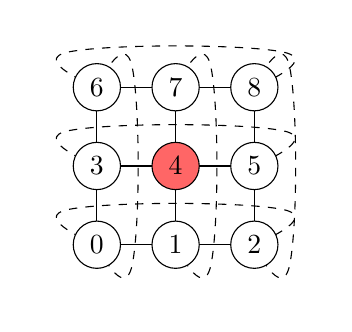
\begin{tikzpicture}

      \draw(0,0) -- (0,2);
      \draw(1,0) -- (1,2);
      \draw(2,0) -- (2,2);

      \draw [black, dashed] plot [smooth, tension=0.8] coordinates { (0,0) (0.45,-0.25) (0.45,2.25) (0,2)};
      \draw [black, dashed] plot [smooth, tension=0.8] coordinates { (1,0) (1.45,-0.25) (1.45,2.25) (1,2)};
      \draw [black, dashed] plot [smooth, tension=0.8] coordinates { (2,0) (2.45,-0.25) (2.45,2.25) (2,2)};


      \draw(0,0) -- (2,0);
      \draw(0,1) -- (2,1);
      \draw(0,2) -- (2,2);

      \draw [black, dashed] plot [smooth, tension=0.8] coordinates { (0,0) (-0.35,0.45) (2.35,0.45) (2,0)};
      \draw [black, dashed] plot [smooth, tension=0.8] coordinates { (0,1) (-0.35,1.45) (2.35,1.45) (2,1)};
      \draw [black, dashed] plot [smooth, tension=0.8] coordinates { (0,2) (-0.35,2.45) (2.35,2.45) (2,2)};

      \draw[black,fill=white](0,0) circle (0.3) node {0};
      \draw[black,fill=white](1,0) circle (0.3) node {1};
      \draw[black,fill=white](2,0) circle (0.3) node {2};

      \draw[black,fill=white](0,1) circle (0.3) node {3};
      \draw[black,fill=red!60](1,1) circle (0.3) node {4};
      \draw[black,fill=white](2,1) circle (0.3) node {5};

      \draw[black,fill=white](0,2) circle (0.3) node {6};
      \draw[black,fill=white](1,2) circle (0.3) node {7};
      \draw[black,fill=white](2,2) circle (0.3) node {8};

    \end{tikzpicture}
  \end{center}
  \caption{n=3-ös rács}
  \label{fig:3Racs}
\end{figure}

\begin{align}
  N = n^2 = 9
\end{align}

\begin{align}
  S_{\text{left}} = I_3 \otimes U_3 =
  \begin{pmatrix}
    0                  & \textcolor{red}{1} & 0                  & 0                  & 0                  & 0                  & 0                  & 0                  & 0                  \\
    0                  & 0                  & \textcolor{red}{1} & 0                  & 0                  & 0                  & 0                  & 0                  & 0                  \\
    \textcolor{red}{1} & 0                  & 0                  & 0                  & 0                  & 0                  & 0                  & 0                  & 0                  \\
    0                  & 0                  & 0                  & 0                  & \textcolor{red}{1} & 0                  & 0                  & 0                  & 0                  \\
    0                  & 0                  & 0                  & 0                  & 0                  & \textcolor{red}{1} & 0                  & 0                  & 0                  \\
    0                  & 0                  & 0                  & \textcolor{red}{1} & 0                  & 0                  & 0                  & 0                  & 0                  \\
    0                  & 0                  & 0                  & 0                  & 0                  & 0                  & 0                  & \textcolor{red}{1} & 0                  \\
    0                  & 0                  & 0                  & 0                  & 0                  & 0                  & 0                  & 0                  & \textcolor{red}{1} \\
    0                  & 0                  & 0                  & 0                  & 0                  & 0                  & \textcolor{red}{1} & 0                  & 0
  \end{pmatrix}
\end{align}

\begin{align}
  S_{\text{right}} = I_3 \otimes L_3 =
  \begin{pmatrix}
    0                  & 0                  & \textcolor{red}{1} & 0                  & 0                  & 0                  & 0                  & 0                  & 0                  \\
    \textcolor{red}{1} & 0                  & 0                  & 0                  & 0                  & 0                  & 0                  & 0                  & 0                  \\
    0                  & \textcolor{red}{1} & 0                  & 0                  & 0                  & 0                  & 0                  & 0                  & 0                  \\
    0                  & 0                  & 0                  & 0                  & 0                  & \textcolor{red}{1} & 0                  & 0                  & 0                  \\
    0                  & 0                  & 0                  & \textcolor{red}{1} & 0                  & 0                  & 0                  & 0                  & 0                  \\
    0                  & 0                  & 0                  & 0                  & \textcolor{red}{1} & 0                  & 0                  & 0                  & 0                  \\
    0                  & 0                  & 0                  & 0                  & 0                  & 0                  & 0                  & 0                  & \textcolor{red}{1} \\
    0                  & 0                  & 0                  & 0                  & 0                  & 0                  & \textcolor{red}{1} & 0                  & 0                  \\
    0                  & 0                  & 0                  & 0                  & 0                  & 0                  & 0                  & \textcolor{red}{1} & 0
  \end{pmatrix}
\end{align}


\begin{align}
  S_{\text{down}} = U_3^3 = U_3 \otimes I_3 =
  \begin{pmatrix}
    0                  & 0                  & 0                  & \textcolor{red}{1} & 0                  & 0                  & 0                  & 0                  & 0                  \\
    0                  & 0                  & 0                  & 0                  & \textcolor{red}{1} & 0                  & 0                  & 0                  & 0                  \\
    0                  & 0                  & 0                  & 0                  & 0                  & \textcolor{red}{1} & 0                  & 0                  & 0                  \\
    0                  & 0                  & 0                  & 0                  & 0                  & 0                  & \textcolor{red}{1} & 0                  & 0                  \\
    0                  & 0                  & 0                  & 0                  & 0                  & 0                  & 0                  & \textcolor{red}{1} & 0                  \\
    0                  & 0                  & 0                  & 0                  & 0                  & 0                  & 0                  & 0                  & \textcolor{red}{1} \\
    \textcolor{red}{1} & 0                  & 0                  & 0                  & 0                  & 0                  & 0                  & 0                  & 0                  \\
    0                  & \textcolor{red}{1} & 0                  & 0                  & 0                  & 0                  & 0                  & 0                  & 0                  \\
    0                  & 0                  & \textcolor{red}{1} & 0                  & 0                  & 0                  & 0                  & 0                  & 0
  \end{pmatrix}
\end{align}


\begin{align}
  S_{\text{up}} = L_3^3 = L_3 \otimes I_3 =
  \begin{pmatrix}
    0                  & 0                  & 0                  & 0                  & 0                  & 0                  & \textcolor{red}{1} & 0                  & 0                  \\
    0                  & 0                  & 0                  & 0                  & 0                  & 0                  & 0                  & \textcolor{red}{1} & 0                  \\
    0                  & 0                  & 0                  & 0                  & 0                  & 0                  & 0                  & 0                  & \textcolor{red}{1} \\
    \textcolor{red}{1} & 0                  & 0                  & 0                  & 0                  & 0                  & 0                  & 0                  & 0                  \\
    0                  & \textcolor{red}{1} & 0                  & 0                  & 0                  & 0                  & 0                  & 0                  & 0                  \\
    0                  & 0                  & \textcolor{red}{1} & 0                  & 0                  & 0                  & 0                  & 0                  & 0                  \\
    0                  & 0                  & 0                  & \textcolor{red}{1} & 0                  & 0                  & 0                  & 0                  & 0                  \\
    0                  & 0                  & 0                  & 0                  & \textcolor{red}{1} & 0                  & 0                  & 0                  & 0                  \\
    0                  & 0                  & 0                  & 0                  & 0                  & \textcolor{red}{1} & 0                  & 0                  & 0
  \end{pmatrix}
\end{align}

\begin{align}
  X_{\text{head}} =
  \begin{pmatrix}
    1 & 0 \\
    0 & 0
  \end{pmatrix}
\end{align}

\begin{align}
  X_{\text{tail}} =
  \begin{pmatrix}
    0 & 0 \\
    0 & 1
  \end{pmatrix}
\end{align}


\begin{align}
  S =
  (S_{\text{up}} S_{\text{left}}) \otimes (X_{\text{head}} \otimes X_{\text{head}}) +    \\
  (S_{\text{up}}  S_{\text{right}}) \otimes (X_{\text{head}} \otimes X_{\text{tail}}) +  \\
  (S_{\text{down}}  S_{\text{left}}) \otimes (X_{\text{tail}} \otimes X_{\text{head}}) + \\
  (S_{\text{down}} S_{\text{right}}) \otimes (X_{\text{tail}} \otimes X_{\text{tail}})
\end{align}

\begin{align}
  C_4 = H^{\otimes2} = \frac{1}{2}
  \begin{pmatrix}
    1 & 1  & 1  & 1  \\
    1 & -1 & 1  & -1 \\
    1 & 1  & -1 & -1 \\
    1 & -1 & -1 & 1
  \end{pmatrix}
\end{align}

\begin{align}
  U = S  (I_9 \otimes C_4)
\end{align}

\begin{align}
  U =
  ((S_{\text{up}}  S_{\text{left}}) \otimes (X_{\text{head}} \otimes X_{\text{head}}) +  \\
  (S_{\text{up}} S_{\text{right}}) \otimes (X_{\text{head}} \otimes X_{\text{tail}}) +   \\
  (S_{\text{down}}  S_{\text{left}}) \otimes (X_{\text{tail}} \otimes X_{\text{head}}) + \\
  (S_{\text{down}} S_{\text{right}}) \otimes (X_{\text{tail}} \otimes X_{\text{tail}}))
  (I_9 \otimes C_4)
\end{align}

\definition[Tenzorszorzás azonosság: mátrix szorzással disztibutív]

Bal oldalt 9*9-es, jobb oldalt 4*4-es mátrixok vannak.

\begin{align}
  U =
  (S_{\text{up}}  S_{\text{left}}) \otimes ((X_{\text{head}} \otimes X_{\text{head}})  C_4) +   \\
  (S_{\text{up}}  S_{\text{right}}) \otimes ((X_{\text{head}} \otimes X_{\text{tail}}) C_4) +   \\
  (S_{\text{down}}  S_{\text{left}}) \otimes ((X_{\text{tail}} \otimes X_{\text{head}})  C_4) + \\
  (S_{\text{down}}  S_{\text{right}}) \otimes ((X_{\text{tail}} \otimes X_{\text{tail}}) C_4)
\end{align}

\begin{align}
  C_4 = C_2 \otimes C_2
\end{align}

\begin{align}
  U =
  (S_{\text{up}}  S_{\text{left}}) \otimes ((X_{\text{head}} \otimes X_{\text{head}}) (C_2 \otimes C_2)) +   \\
  (S_{\text{up}}  S_{\text{right}}) \otimes ((X_{\text{head}} \otimes X_{\text{tail}}) (C_2 \otimes C_2)) +  \\
  (S_{\text{down}}  S_{\text{left}}) \otimes ((X_{\text{tail}} \otimes X_{\text{head}}) (C_2 \otimes C_2)) + \\
  (S_{\text{down}}  S_{\text{right}}) \otimes ((X_{\text{tail}} \otimes X_{\text{tail}}) (C_2 \otimes C_2))
\end{align}

\definition[Tenzorszorzás azonosság: mátrix szorzással disztibutív]

\begin{align}
  U =
  (S_{\text{up}}  S_{\text{left}}) \otimes (((X_{\text{head}}C_2) \otimes (X_{\text{head}}C_2))) +   \\
  (S_{\text{up}}  S_{\text{right}}) \otimes (((X_{\text{head}}C_2) \otimes (X_{\text{tail}}C_2))) +  \\
  (S_{\text{down}}  S_{\text{left}}) \otimes (((X_{\text{tail}}C_2) \otimes (X_{\text{head}}C_2))) + \\
  (S_{\text{down}}  S_{\text{right}}) \otimes (((X_{\text{tail}}C_2) \otimes (X_{\text{tail}}C_2)))
\end{align}

\definition[Tenzorszorzás azonosság: asszociatív]


\begin{align}
  U =
  (S_{\text{up}}  S_{\text{left}}) \otimes (X_{\text{head}}C_2) \otimes (X_{\text{head}}C_2) +   \\
  (S_{\text{up}}  S_{\text{right}}) \otimes (X_{\text{head}}C_2) \otimes (X_{\text{tail}}C_2) +  \\
  (S_{\text{down}}  S_{\text{left}}) \otimes (X_{\text{tail}}C_2) \otimes (X_{\text{head}}C_2) + \\
  (S_{\text{down}}  S_{\text{right}}) \otimes (X_{\text{tail}}C_2) \otimes (X_{\text{tail}}C_2)
\end{align}


\definition[Tenzorszorzás Lemma?]


\begin{align}
  S = ((S_{\text{up}} \otimes  X_{\text{head}} \otimes I) +
  (S_{\text{down}} \otimes X_{\text{tail}} \otimes I))
  ((S_{\text{left}} \otimes I \otimes X_{\text{head}}) +
  (S_{\text{right}} \otimes I \otimes  X_{\text{tail}} ))
\end{align}


% \begin{align}
%   U =
%   ((S_{\text{up}}  S_{\text{left}}) \otimes I_2) (I_9 \otimes (X_{\text{head}}C_2)) \otimes (X_{\text{head}}C_2) +   \\
%   ((S_{\text{up}}  S_{\text{right}}) \otimes I_2) (I_9 \otimes (X_{\text{head}}C_2)) \otimes (X_{\text{tail}}C_2) +  \\
%   ((S_{\text{down}}  S_{\text{left}}) \otimes I_2) (I_9 \otimes (X_{\text{tail}}C_2)) \otimes (X_{\text{head}}C_2) + \\
%   ((S_{\text{down}}  S_{\text{right}}) \otimes I_2) (I_9 \otimes (X_{\text{tail}}C_2)) \otimes (X_{\text{tail}}C_2)
% \end{align}